\documentclass[12pt,a4paper,twoside,openright]{report}
\let\openright=\cleardoublepage



%%% Choose a language %%%

\newif\ifEN
\ENtrue   % uncomment this for english
%\ENfalse   % uncomment this for czech

%%% Configuration of the title page %%%

\def\ThesisTitleStyle{mff} % MFF style
%\def\ThesisTitleStyle{cuni} % uncomment for old-style with cuni.cz logo
%\def\ThesisTitleStyle{natur} % uncomment for nature faculty logo

\def\UKFaculty{Faculty of Mathematics and Physics}
%\def\UKFaculty{Faculty of Science}

\def\UKName{Charles University in Prague} % this is not used in the "mff" style

% Thesis type names, as used in several places in the title
\def\ThesisTypeTitle{\ifEN BACHELOR THESIS \else BAKALÁŘSKÁ PRÁCE \fi}
%\def\ThesisTypeTitle{\ifEN MASTER THESIS \else DIPLOMOVÁ PRÁCE \fi}
%\def\ThesisTypeTitle{\ifEN RIGOROUS THESIS \else RIGORÓZNÍ PRÁCE \fi}
%\def\ThesisTypeTitle{\ifEN DOCTORAL THESIS \else DISERTAČNÍ PRÁCE \fi}
\def\ThesisGenitive{\ifEN bachelor \else bakalářské \fi}
%\def\ThesisGenitive{\ifEN master \else diplomové \fi}
%\def\ThesisGenitive{\ifEN rigorous \else rigorózní \fi}
%\def\ThesisGenitive{\ifEN doctoral \else disertační \fi}
\def\ThesisAccusative{\ifEN bachelor \else bakalářskou \fi}
%\def\ThesisAccusative{\ifEN master \else diplomovou \fi}
%\def\ThesisAccusative{\ifEN rigorous \else rigorózní \fi}
%\def\ThesisAccusative{\ifEN doctoral \else disertační \fi}



%%% Fill in your details %%%

% (Note: \xxx is a "ToDo label" which makes the unfilled visible. Remove it.)
\def\ThesisTitle{Implicit Information Extraction from News Stories}
\def\ThesisAuthor{Hynek Kydlíček}
\def\YearSubmitted{2023}

% department assigned to the thesis
\def\Department{Institute of Formal and Applied Linguistics}
% Is it a department (katedra), or an institute (ústav)?
\def\DeptType{Institute}

\def\Supervisor{Mgr. Jindřich Libovický, Ph.D.}
\def\SupervisorsDepartment{Institute of Formal and Applied Linguistics}

% Study programme and specialization
\def\StudyProgramme{Computer Science}
\def\StudyBranch{Artificial Intelligence Bc.}

\def\Dedication{%
I would like to thank my supervisor Mgr. Jindřich Libovický, Ph.D. for his guidance and support throughout the whole process.
I would also like to thank my family and friends for their support and encouragement.
}

\def\AbstractEN{%
This work deals with information extraction from Czech News Stories. We focus on 4 tasks:
Publishing server, Article's category, Author's textual gender and Publication day of week. 
As no dataset for these tasks exists, this work presents a new extensive dataset of 1.5M Czech news articles
with various metadata. With the dataset, we also publish a new tool C'monCrawl for extracting resources from CommonCrawl
archive. Tasks are then solved using various machine learning methods mainly based on Transformer architecture.
Our work sets strong baseline results on the said dataset allowing for further research in the field.
}

\def\AbstractCS{%
Tato práce se zabývá extrakcí informací z českých zpravodajských článků. Zaměřujeme se na 4 úlohy:
Vydavatelský server, kategorie článku, textový gender autra a den vydání.
Protože pro tyto úlohy neexistuje žádná datová sada, představuje tato práce novou rozsáhlou datovout sadu
čítající 1,5 milionu českých zpravodajských článků s rozličnými metadaty.
Spolu s datovou sadou publikujeme také nový nástroj C'monCrawl pro extrakci zdrojů z CommonCrawl archivu.
archivu. Úlohy jsou pak řešeny pomocí různých metod strojového učení založených především na architektuře Transformer.
Naše práce představuje silný základný výsledek na uvedené datové sadě, který umožňuje další výzkum v této oblasti.
}

% 3 to 5 keywords (recommended), each enclosed in curly braces.
% Keywords are useful for indexing and searching for the theses by topic.
\def\Keywords{%
{Information Extraction}, {Server}, {Category}, {Gender} 
{Day Of Week}, {C'monCrawl}, {Czech News Dataset}
}

% If your abstracts are long and do not fit in the infopage, you can make the
% fonts a bit smaller by this setting. (Also, you should try to compress your abstract more.)
% Alternatively, consider increasing the size of the page by uncommenting the
% geometry modification in thesis.tex.
\def\InfoPageFont{}
%\def\InfoPageFont{\small}  %uncomment to decrease font size

\ifEN\relax\else
% If you are writing a czech thesis, you additionally need to fill in the
% english translation of the metadata here!
\def\ThesisTitleEN{\xxx{Thesis title in English}}
\def\DepartmentEN{\xxx{Name of the department in English}}
\def\DeptTypeEN{\xxx{Department}}
\def\SupervisorsDepartmentEN{\xxx{Superdepartment}}
\def\StudyProgrammeEN{\xxx{study programme}}
\def\StudyBranchEN{\xxx{study branch}}
\def\KeywordsEN{%
\xxx{{key} {words}}
}
\fi


\usepackage[a-2u]{pdfx}

\ifEN\else\usepackage[czech,shorthands=off]{babel}\fi
\usepackage[utf8]{inputenc}
\usepackage[T1]{fontenc}

% See https://en.wikipedia.org/wiki/Canons_of_page_construction before
% modifying the size of printable area. LaTeX defaults are great.
% If you feel it would help anything, you can enlarge the printable area a bit:
%\usepackage[textwidth=390pt,textheight=630pt]{geometry}
% The official recommendation expands the area quite a bit (looks pretty harsh):
%\usepackage[textwidth=145mm,textheight=247mm]{geometry}

%%% FONTS %%%
\usepackage{lmodern} % TeX "original" (this sets up the latin mono)

% Optionally choose an override for the main font for typesetting
\usepackage[mono=false]{libertinus} % popular for comp-sci (ACM uses this)
%\usepackage{tgschola} % Schoolbook-like (gives a bit of historic feel)
%\usepackage[scale=0.96]{tgpagella} % Palladio-like (popular in formal logic).

% Optionally choose a custom sans-serif fonts (e.g. for figures and tables).
% Default sans-serif font is usually Latin Modern Sans. Some font packages
% (e.g. libertinus) replace that with a better matching sans-serif font.
%\usepackage{tgheros} % recommended and very readable (Helvetica-like)
%\usepackage{FiraSans} % looks great
% DO NOT typeset the main text in sans-serif font!
% The serifs make the text easily readable on the paper.

% IMPORTANT FONT NOTE: Some fonts require additional PDF/A conversion using
% the pdfa.sh script. These currently include only 'tgpagella'; but various
% other fonts from the texlive distribution need that too (mainly the Droid
% font family).


% some useful packages
\usepackage{microtype}
\usepackage{amsmath,amsfonts,amsthm,bm}
\usepackage{graphicx}
\usepackage{xcolor}
\usepackage{booktabs}
\usepackage{caption}
\usepackage{floatrow}

% for enum ref
\usepackage{enumitem}
% load bibliography tools
\usepackage[backend=bibtex,natbib,style=numeric,sorting=none]{biblatex}
% alternative with alphanumeric citations (more informative than numbers):
% \usepackage[backend=bibtex,natbib,style=alphabetic]{biblatex}
% \usepackage[]{biblatex}
%
% alternatives that conform to iso690
% (iso690 is not formally required on MFF, but may help elsewhere):
%\usepackage[backend=bibtex,natbib,style=iso-numeric,sorting=none]{biblatex}
%\usepackage[backend=bibtex,natbib,style=iso-alphabetic]{biblatex}
%
% additional option choices:
%  - add `giveninits=true` to typeset "E. A. Poe" instead of full Edgar Allan
%  - `terseinits=true` additionaly shortens it to nature-like "Poe EA"
%  - add `maxnames=10` to limit (or loosen) the maximum number of authors in
%    bibliography entry before shortening to `et al.` (useful when referring to
%    book collections that may have hundreds of authors)
%  - for additional flexibility (e.g. multiple reference sections, etc.),
%    remove `backend=bibtex` and compile with `biber` instead of `bibtex` (see
%    Makefile)
%  - `sorting=none` causes the bibliography list to be ordered by the order of
%    citation as they appear in the text, which is usually the desired behavior
%    with numeric citations. Additionally you can use a style like
%    `numeric-comp` that compresses the long lists of citations such as
%    [1,2,3,4,5,6,7,8] to simpler [1--8]. This is especially useful if you plan
%    to add tremendous amounts of citations, as usual in life sciences and
%    bioinformatics.
%  - if you don't like the "In:" appearing in the bibliography, use the
%    extended style (`ext-numeric` or `ext-alphabetic`), and add option
%    `articlein=false`.
%
% possibly reverse the names of the authors with the default styles:
%\DeclareNameAlias{default}{family-given}

% load the file with bibliography entries
\addbibresource{refs.bib}

% remove this if you won't use fancy verbatim environments
\usepackage{fancyvrb}

% remove this if you won't typeset TikZ graphics
\usepackage{tikz}
\usetikzlibrary{positioning, shapes.multipart} %add libraries as needed (shapes, decorations, ...)

% remove this if you won't typeset any pseudocode
\usepackage{algpseudocode}
\usepackage{algorithm}

% remove this if you won't list any source code
\usepackage{listings}


\hypersetup{unicode}
\hypersetup{breaklinks=true}

\usepackage[noabbrev]{cleveref}


% various forms of TODOs (you should remove this before submitting)
\usepackage[textsize=tiny, backgroundcolor=yellow!25, linecolor=black!25]{todonotes}
\newcommand{\xxx}[1]{\textcolor{red!}{#1}}

 % remove this before compiling the final version


% use this for typesetting a chapter without a number, e.g. intro and outro
\def\chapwithtoc#1{
\chapter*{#1}
\addcontentsline{toc}{chapter}{#1}
}

% If there is a line/figure overflowing into page margin, this will make the
% problem evident by drawing a thick black line at the overflowing spot. You
% should not disable this.
\overfullrule=3mm

% The maximum stretching of a space. Increasing this makes the text a bit more
% sloppy, but may prevent the overflows by moving words to next line.
\emergencystretch=1em

\ifEN
\theoremstyle{plain}
\newtheorem{thm}{Theorem}
\newtheorem{lemma}[thm]{Lemma}
\newtheorem{claim}[thm]{Claim}
\newtheorem{defn}{Definition}
\theoremstyle{remark}
\newtheorem*{cor}{Corollary}
\else
\theoremstyle{plain}
\newtheorem{thm}{Věta}
\newtheorem{lemma}{Lemma}
\newtheorem{claim}{Tvrzení}
\newtheorem{defn}{Definice}
\theoremstyle{remark}
\newtheorem*{cor}{Důsledek}
\fi

\newenvironment{myproof}{
  \par\medskip\noindent
  \textit{\ifEN Proof \else Důkaz \fi}.
}{
\newline
\rightline{$\qedsymbol$}
}

% real/natural numbers
\newcommand{\R}{\mathbb{R}}
\newcommand{\N}{\mathbb{N}}

% asymptotic complexity
\newcommand{\asy}[1]{\mathcal{O}(#1)}

% listings and default lstlisting config (remove if unused)
\DeclareNewFloatType{listing}{}
\floatsetup[listing]{style=ruled}

\DeclareCaptionStyle{thesis}{style=base,font={small,sf},labelfont=bf,labelsep=quad}
\captionsetup{style=thesis}
\captionsetup[algorithm]{style=thesis,singlelinecheck=off}
\captionsetup[listing]{style=thesis,singlelinecheck=off}

% Uncomment for table captions on top. This is sometimes recommended by the
% style guide, and even required for some publication types.
%\floatsetup[table]{capposition=top}
%
% (Opinionated rant:) Captions on top are not "compatible" with the general
% guideline that the tables should be formatted to be quickly visually
% comprehensible and *beautiful* in general (like figures), and that the table
% "head" row (with column names) should alone communicate most of the content
% and interpretation of the table. If you just need to show a long boring list
% of numbers (because you have to), either put some effort into showing the
% data in an attractive figure-table, or move the data to an attachment and
% refer to it, so that the boredom does not impact the main text flow.
%
% You can make the top-captions look much less ugly by aligning the widths of
% the caption and the table, with setting `framefit=yes`, as shown below.  This
% additionally requires some extra markup in your {table} environments; see the
% comments in the example table in `ch2.tex` for details.
%\floatsetup[table]{capposition=top,framefit=yes}

\ifEN\floatname{listing}{Listing}
\else\floatname{listing}{Výpis kódu}\fi
\lstset{ % use this to define styling for any other language
  language=C++,
  tabsize=2,
  showstringspaces=false,
  basicstyle=\footnotesize\tt\color{black!75},
  identifierstyle=\bfseries\color{black},
  commentstyle=\color{green!50!black},
  stringstyle=\color{red!50!black},
  keywordstyle=\color{blue!75!black}}

% Czech versions of the used cleveref references (It's not as convenient as in
% English because of declension, cleveref is limited to sg/pl nominative. Use
% plain \ref to dodge that.)
\ifEN\relax\else
\crefname{chapter}{kapitola}{kapitoly}
\Crefname{chapter}{Kapitola}{Kapitoly}
\crefname{section}{sekce}{sekce}
\Crefname{section}{Sekce}{Sekce}
\crefname{subsection}{sekce}{sekce}
\Crefname{subsection}{Sekce}{Sekce}
\crefname{subsubsection}{sekce}{sekce}
\Crefname{subsubsection}{Sekce}{Sekce}
\crefname{figure}{obrázek}{obrázky}
\Crefname{figure}{Obrázek}{Obrázky}
\crefname{table}{tabulka}{tabulky}
\Crefname{table}{Tabulka}{Tabulky}
\crefname{listing}{výpis}{výpisy}
\Crefname{listing}{Výpis}{Výpisy}
\floatname{algorithm}{Algoritmus}
\crefname{algorithm}{algoritmus}{algoritmy}
\Crefname{algorithm}{Algoritmus}{Algoritmy}
\newcommand{\crefpairconjunction}{ a~}
\newcommand{\crefrangeconjunction}{ a~}
\fi
 % use this file for various custom definitions


\begin{document}

% the layout is mandatory, edit only in dire circumstances

\pagestyle{empty}
\hypersetup{pageanchor=false}
\begin{center}

% top part of the layout, this actually differs between faculties

\def\ThesisTitleXmff{%
  \ifEN
    \centerline{\mbox{
\includegraphics[width=166mm]{img/logo-en.pdf}}}
  \else
    \centerline{\mbox{
\includegraphics[width=166mm]{img/logo-cs.pdf}}}
  \fi
  \vspace{-8mm}\vfill%
  {\bf\Large\ThesisTypeTitle}
  \vfill%
  {\LARGE\ThesisAuthor}\par
  \vspace{15mm}%
  {\LARGE\bfseries\ThesisTitle}
  \vfill%
  \Department}
\def\ThesisTitleCuniLogo#1{%
  {\large\UKName\par\medskip\par\UKFaculty }
  \vfill%
  {\bf\Large\ThesisTypeTitle}
  \vfill%
  \includegraphics[width=70mm]{#1}
  \vfill%
  {\LARGE\ThesisAuthor}\par
  \vspace{15mm}%
  {\LARGE\bfseries\ThesisTitle}
  \vfill%
  \Department\par}
\def\ThesisTitleXcuni{\ThesisTitleCuniLogo{img/uklogo.pdf}}
\def\ThesisTitleXnatur{\ThesisTitleCuniLogo{img/naturlogo.pdf}}

% choose the correct page and print it
\csname ThesisTitleX\ThesisTitleStyle\endcsname
% latex corner: X is the new @

\vfill

{
\centerline{\vbox{\halign{\hbox to 0.45\hsize{\hfil #}&\hskip 0.5em\parbox[t]{0.45\hsize}{\raggedright #}\cr
\ifEN Supervisor of the \ThesisGenitive thesis:
\else Vedoucí \ThesisGenitive práce: \fi
& \Supervisor \cr
\noalign{\vspace{2mm}}
\ifEN Study programme: \else Studijní program: \fi
& \StudyProgramme \cr
\noalign{\vspace{2mm}}
\ifEN Study branch: \else Studijní obor: \fi
& \StudyBranch \cr
}}}}

\vfill

\ifEN Prague \else Praha \fi
\YearSubmitted

\end{center}

\newpage

% remember to sign this!
\openright
\hypersetup{pageanchor=true}
\pagestyle{plain}
\pagenumbering{roman}
\vglue 0pt plus 1fill

\ifEN
\noindent
I declare that I carried out this \ThesisAccusative thesis independently, and only with the cited
sources, literature and other professional sources. It has not been used to obtain another
or the same degree.
\else
\noindent
Prohlašuji, že jsem tuto \ThesisAccusative práci vypracoval(a) samostatně a výhradně
s~použitím citovaných pramenů, literatury a dalších odborných zdrojů.
Tato práce nebyla využita k získání jiného nebo stejného titulu.
\fi

\ifEN
\medskip\noindent
I understand that my work relates to the rights and obligations under the Act No.~121/2000 Sb.,
the Copyright Act, as amended, in particular the fact that the Charles
University has the right to conclude a license agreement on the use of this
work as a school work pursuant to Section 60 subsection 1 of the Copyright~Act.
\else
\medskip\noindent
Beru na~vědomí, že se na moji práci vztahují práva a povinnosti vyplývající
ze zákona č. 121/2000 Sb., autorského zákona v~platném znění, zejména skutečnost,
že Univerzita Karlova má právo na~uzavření licenční smlouvy o~užití této
práce jako školního díla podle §60 odst. 1 autorského zákona.
\fi

\vspace{10mm}


\ifEN
\hbox{\hbox to 0.5\hsize{%
In \hbox to 6em{\dotfill} date \hbox to 6em{\dotfill}
\hss}\hbox to 0.5\hsize{\dotfill\quad}}
\smallskip
\hbox{\hbox to 0.5\hsize{}\hbox to 0.5\hsize{\hfil Author's signature\hfil}}
\else
\hbox{\hbox to 0.5\hsize{%
V \hbox to 6em{\dotfill} dne \hbox to 6em{\dotfill}
\hss}\hbox to 0.5\hsize{\dotfill\quad}}
\smallskip
\hbox{\hbox to 0.5\hsize{}\hbox to 0.5\hsize{\hfil Podpis autora\hfil}}
\fi

\vspace{20mm}
\newpage

% dedication

\openright

\noindent
\Dedication

\newpage

% mandatory information page

\openright

\vbox to 0.49\vsize{\InfoPageFont
\setlength\parindent{0mm}
\setlength\parskip{5mm}

\ifEN Title: \else Název práce: \fi
\ThesisTitle

\ifEN Author: \else Autor: \fi
\ThesisAuthor

\DeptType:
\Department

\ifEN Supervisor: \else Vedoucí bakalářské práce: \fi
\Supervisor, \SupervisorsDepartment

\ifEN Abstract: \AbstractEN \else Abstrakt: \AbstractCS \fi

\ifEN Keywords: \else Klíčová slova: \fi
\Keywords

\vss}\ifEN\relax\else\nobreak\vbox to 0.49\vsize{\InfoPageFont
\setlength\parindent{0mm}
\setlength\parskip{5mm}

Title:
\ThesisTitleEN

Author:
\ThesisAuthor

\DeptTypeEN:
\DepartmentEN

Supervisor:
\Supervisor, \SupervisorsDepartmentEN

Abstract:
\AbstractEN

Keywords:
\KeywordsEN

\vss}
\fi

\newpage

\openright
\pagestyle{plain}
\pagenumbering{arabic}
\setcounter{page}{1}


\tableofcontents

\chapwithtoc{Introduction}
Every day there are millions of articles published on the internet. Various authors write those
with different backgrounds and opinions. Their goal is, however, the same: to convey the information to the reader.
While the information is usually explicit there are some cases when it is implicit. Such implicit information 
is usually intentionally used to shape the reader's opinion. However, it's also possible
that the author inserts such implicit information unintentionally. It could
be the result of the author's background or state of the world at the time of writing.
The author's texts might be more pessimistic at the start of the week while more optimistic before the weekend.
It might also be possible that women write articles slightly differently than men do.
We thus ask ourselves the following question:
\begin{quote}
    \textit{Which and how much implicit information can be extracted from the news articles?}
\end{quote}

As there could be an infinite amount of such fingerprints, we decided to narrow the scope of our research to only:
\begin{enumerate}
    \item The category of the article
    \item Infered gender of article author's name
    \item Day of week when the article was published
    \item News server where the article was published
\end{enumerate}
We also had to narrow the domain of our research to news articles in Czech.

\section*{Related Work}
With the rise of Natural Language Processing (NLP) and Machine Learning (ML)
there has been a lot of research on implicit information in textual content.
In particular, sentiment analysis and text classification have been researched by many.
Most notably, \cite{joulinBagTricksEfficient2016} showed that a simple bag of words approach
with a few hidden layers could achieve state-of-the-art (SOTA) results while being very fast and straightforward.
\cite{zhangTextUnderstandingScratch2016} inspired by the usage of convolutional neural networks in image classification,
proposed a similar approach for text classification with excellent results.
In recent years, state-of-the-art has been achieved by the transformer models \cite{vaswaniAttentionAllYou2017d}.
Such an approach was used in \cite{devlinBERTPretrainingDeep2019a} where the authors achieved SOTA results on
all the tasks of GLUE benchmark \cite{wangGLUEMultiTaskBenchmark2019}, which among others, includes 
sentiment analysis task. Inspired by these results \cite{sunHowFineTuneBERT2020} further investigated possibilities
of fine-tuning BERT creating eight SOTA results on text classification tasks.

\section*{Our approach}
As no dataset with needed labels exists we created one of the most extensive datasets of Czech news articles. 
With more than 1.5 million articles it is on par with \cite{sidoCzertCzechBERTlike2021}.
while containing more metadata about the articles.

To test human ability on the tasks we took a subset of the dataset and tested human performance.

As for machine learning models, we fine-tuned the \textit{RobeCzech} (\cite{strakaRobeCzechCzechRoBERTa2021}),
and the \textit{Fernet-News} (\cite{leheckaComparisonCzechTransformers2021}) models. 
We have also used GPT-3 \cite{brownLanguageModelsAre2020b} to test its capabilities.

\section*{Structure of the thesis}
We start with the introduction to text classification, then provide readers with the necessary background knowledge
to understand the models we will use. We proceed to describe dataset creation and its properties.
Next, we describe the experiments we conducted and their results. Finally, we conclude with a summary of our findings.
\chapter{Text classification}
Information extraction from the text can be stated as a text classification task.
Given a text, we want to assign a class it belongs to.
The class can be anything, from the text's category to the text's sentiment or the author's age.
Depending on the number of classes, we can distinguish between \textbf{binary} (2) and \textbf{multiclass} (2+) classification.
We might want to classify the text by multiple labels; we thus also distinguish between \textbf{single-label}
and \textbf{multi-label} classification.

Therefore, we can rephrase our research question as a \textbf{single-label multiclass text classification of Czech News articles}.
To avoid ambiguity, we will refer to a single news article text as a \textbf{document} going forward.

\section{Evaluation Metrics}
\label{sec:metrics}
To assess performance, we need to define some metrics.
We start by defining metrics for binary classification and then extend them to multiclass classification.

In Binary classification, we have two classes; positive and negative. Thus we can have four possible outcomes:
\begin{enumerate}
    \item \ac{tp} - prediction positive, label positive
    \item \ac{tn} - prediction negative, label negative
    \item \ac{fn} - prediction negative, label positive
    \item \ac{fp} - prediction positive, label negative
\end{enumerate}

The most basic metric is accuracy, which is defined as
\begin{equation*}
    \label{eq:accuracy}
    \operatorname{Accuracy} = \frac{\mathrm{TP} + \mathrm{TN}}{\mathrm{TP} + \mathrm{TN} + \mathrm{FP} + \mathrm{FN}}
\end{equation*}
However, accuracy often fails to capture the whole picture.
Let's consider a dataset of 1000 people, where 990 are healthy and 10 are sick.
Such a dataset is called \textbf{imbalanced}, as the number of classes is distributed unequally.
We will consider sick people to be positive class and healthy people to be negative class.
On this dataset, we could achieve 99\% accuracy by always predicting that the person is healthy.
Such a model would be useless in practice, as it could not detect sick people.

\subsection{Precision and Recall}
Precision and recall deal with the issue of imbalanced datasets.
They are defined as
\begin{equation*}
    \label{eq:precision}
    \operatorname{Precision} = \frac{\mathrm{TP}}{\mathrm{TP} + \mathrm{FP}}
\end{equation*}
\begin{equation*}
    \label{eq:recall}
    \operatorname{Recall} = \frac{\mathrm{TP}}{\mathrm{TP} + \mathrm{FN}}
\end{equation*}
Considering the same model, we will score 0\% recall and undefined precision.
If we were to increase the recall by always predicting sick, we would achieve 100\% recall and 1\% precision.
A good model should thus have both high precision and recall.

\subsection{$F_{\beta}$ Score}
The $F_{\beta}$ score answers our requirements.
It combines precision and recall into one metric and is defined as
\begin{equation*}
    \label{eq:f1}
    F_{\beta} = (1 + \beta^2) \cdot \frac{\operatorname{Precision} \cdot \operatorname{Recall}}{\beta^2 \cdot \operatorname{Precision} + \operatorname{Recall}}
\end{equation*}
We can control the importance of precision and recall by changing the $\beta$ parameter.

\subsection{Micro and Macro Averaging}
We can use micro and macro averaging to extend the binary metrics to a multiclass case.
In the case of micro averaging, we consider $\mathrm{TP}, \mathrm{TN}, \mathrm{FP}$ and $\mathrm{FN}$ as the sum of respective values for each class.
We then calculate the metrics as before.
In the case of macro averaging, we calculate the metrics for each class and then average them.
This results in treating each class equally irregardless of the number of samples in each class.

\subsection{Interannotator Agreement and Cohen's Kappa}
\label{sec:interannotator}
One can use the \textbf{Cohen's kappa} metric to assess agreement between annotators.
Assume we have two annotators annotating a dataset of $n$ samples with $k$ classes.
Denote class annotated by annotator $i$ to sample $j$ as $c_{ij}$.
Denote a total number of samples annotated by annotator $i$ as class $c$ as $n_{ic}$.
We can then calculate Cohen's kappa as
\begin{equation*}
    \label{eq:kappa}
    \kappa = \frac{p_o - p_e}{1 - p_e}
\end{equation*}
where $p_o$ is the observed agreement and $p_e$ is the expected agreement.
The expected agreement is calculated as
\begin{equation*}
    \label{eq:pe}
    p_e = \sum_{i=1}^k \frac{n_{1i} n_{2i}}{n^2}
\end{equation*}
The observed agreement is calculated as
\begin{equation*}
    \label{eq:po}
    p_o = \frac{1}{n} \sum_{i=1}^n \frac{c_{1i} = c_{2i}}{n}
\end{equation*}
The interpretation of the metric is not well established, as
it is unclear how high the metric should be to be considered good.
\textcite[page 165]{landisMeasurementObserverAgreement1977} suggest the following interpretation:
\begin{itemize}
    \item $\kappa < 0$ - poor agreement
    \item $0 \leq \kappa < 0.2$ - slight agreement
    \item $0.2 \leq \kappa < 0.4$ - fair agreement
    \item $0.4 \leq \kappa < 0.6$ - moderate agreement
    \item $0.6 \leq \kappa < 0.8$ - substantial agreement
    \item $0.8 \leq \kappa < 1$ - almost perfect agreement
\end{itemize}

\section{Notation intermezzo}
\label{sec:notation}
From now on, we will use the following notation:
\begin{itemize}
    \item non-bold lowercase letters (e.g. $x$) will denote a scalar.
    \item bold lowercase letters (e.g. $\mathbf{x}$) will denote a vector.
    \item bold uppercase letters (e.g. $\mathbf{X}$) will denote a matrix.
    \item letters with hat (e.g. $\hat{x}$) will denote a predicted value.
    \item $|V|$ will denote size of set $V$.
\end{itemize}
All vectors are column vectors unless otherwise stated.

\section{Document Representation}
\label{sec:representation}
To train a model, we need to represent the document in a way the model can understand.
Let's consider a dataset $D$ of $N$ documents. We can use the following representations:

\subsection{\acl{bow}}
\label{sec:bow}
One way to represent the document is to encode each word based on the number of occurrences in the document.
Such is an idea of the \acf{bow}. To obtain a \ac{bow} representation, we do the following:
\begin{enumerate}
    \item Tokenize the dataset. This is a process of splitting the text into smaller units called tokens (usually words).
    \item Create a vocabulary $V$ of all the tokens in the dataset.
    \item Represent document $d$ as vector of weights $(C_{d}^1, C_{d}^2, \dots, C_{d}^{|V|})$, where $C_{d}^i$
          is the number of occurrences of token $i$ in document $d$.
\end{enumerate}
This representation allows us to store the dataset as a sparse $N \cdot |V|$ matrix.

\subsection{TF-IDF}
\label{sec:tfidf}
TF-IDF is an extension of the \ac{bow} representation, where we also consider the document's token frequency.
To represent the weight of token $t$ in document $d$, we use the following formula:
\begin{equation*}
    \label{eq:tfidf}
    \operatorname{TF-IDF}(t, d) = \operatorname{TF}(t, d) \cdot \operatorname{IDF}(t)
\end{equation*}
where TF and IDF are defined as
\begin{equation*}
    \label{eq:tf}
    \operatorname{TF}(t, d) = \frac{C_{d}^t}{\sum_{j \in V} C_{d}^{j}}
\end{equation*}
\begin{equation*}
    \label{eq:idf}
    \operatorname{IDF}(t) = \log \frac{|D|}{\sum_{d \in D} (C_{d}^t)}
\end{equation*}


\subsection{Subword Representations}
The problem with preceding representations is that they cannot capture unseen words and require
an extensive vocabulary. To solve this problem, we can use subword representations. Unlike the previous
representations, subword representations are not fixed-sized.

\subsubsection{\acl{bpe}}
\label{sec:bpe}
Popularized by \textcite{sennrichNeuralMachineTranslation2016b}, the \acf{bpe} algorithm is following:
\begin{enumerate}
    \item Split sentences into words by whitespace and punctuation.
    \item Split each word into separate characters and add the special end of the word token.
    \item Initializes the vocabulary with all the found characters and the end of the word token.
    \item Iteratively merge the most frequent pair of characters into a single character.
    \item Stop when the vocabulary size reaches the desired size.
\end{enumerate}
We then use the vocabulary to encode the document as a sequence of token ids.

\subsubsection{WordPiece}
\label{sec:wordpiece}
WordPiece is a modification of \ac{bpe} that uses a different merging
strategy and pre-tokenization. It was first introduced by~\textcite{schusterJapaneseKoreanVoice2012}
and improved by~\textcite{wuGoogleNeuralMachine2016}.
For pre-tokenization, it adds a special token at the beginning instead of the end of the word.
As for the merging strategy, we choose the pair that maximizes the likelihood of the training data when merged.

\subsubsection{\acl{spm}}
\label{sec:spm}
Introduced by~\textcite{kudoSentencePieceSimpleLanguage2018}, \acf{spm} is rather a modular tokenizer than an algorithm.
It unifies the preprocessing and tokenization steps and allows different sub-word algorithms to be used.
Among other things, it also addresses the problem of encoding multiple space characters, which is impossible in the above sub-word algorithms.
It does so by introducing a special token for the space character.


\subsubsection{\acl{bbpe}}
\label{sec:bbpe}
First described by~\textcite{Radford2019LanguageMA}, \acf{bbpe} is a modification of \ac{bpe}.
It doesn't split into words and characters but directly into bytes.
The authors noticed that the encoding was doing suboptimal merges as adding exclamation marks to the end of the words.
To solve this problem, merges can only happen between the same character categories.

\section{\acl{ml} Models}
\label{sec:models}
This section reviews the \ac{ml} models we will use in experiments.
Our intention is not to provide a comprehensive review of text classification approaches.
If the reader is interested in such a work, we recommend work by \textcite{kowsariTextClassificationAlgorithms2019}.
We will not review either \acp{cnn} or \acp{rnn}.
However, we will refer to them and expect the reader to know them.

\subsection{\acl{mlr}}
\label{sec:mlr}
\acf{mlr} is a simple linear model.
The \ac{mlr} with $k$ classes is represented by matrix of weights $\mathbf{W} \in R^{k, d} = (\mathbf{w_1}, \mathbf{w_2}, \dots \mathbf{w_n})^T$
and vector of biases $\mathbf{b} = (\beta_1, \beta_2, \dots \beta_k)$.

Given input $\mathbf{x} \in R^{d}$, with correct class $C_t$, the probability of model predicting class $C_i$ is given by
\begin{align*}
    %% Softmax
    \operatorname{softmax}(\mathbf{z})          & = \frac{e^{z_i}}{\sum_{j=1}^{k} e^{z_j}}     \\
    %% Probability
    P(C_i | \mathbf{x}; \mathbf{W}, \mathbf{b}) & = \sigma(\mathbf{W} \mathbf{x} + \mathbf{b})
\end{align*}
The optimized loss function is cross-entropy loss:
\begin{equation*}
    \mathcal{L}(\mathbf{x};\mathbf{W}, \mathbf{b}) = \log{P(C_t \mathbf{x}; \mathbf{W}, \mathbf{b})}
\end{equation*}

The model is simple, so it can't capture complex relationships between features.
However, it serves as a good baseline model, and unlike later models, it can be easily interpreted.

\subsection{Transformers}
\label{sec:transformers}
Transformers have been first proposed for machine translation by \textcite{vaswaniAttentionAllYou2017d}.
They have since become a \ac{sota} model for many \ac{nlp} tasks, including Text Classification.
The original paper suggested using encoder-decoder architecture due to the nature of the machine translation task.
However, for text classification, there is no need for the decoder. Thus, the architecture can be simplified to only the encoder.
In the following sections by \textbf{transformer}, we will refer to the encoder part of the architecture.

\subsubsection{Architecture}
%import pdf
\begin{figure}[ht]
    \centering
    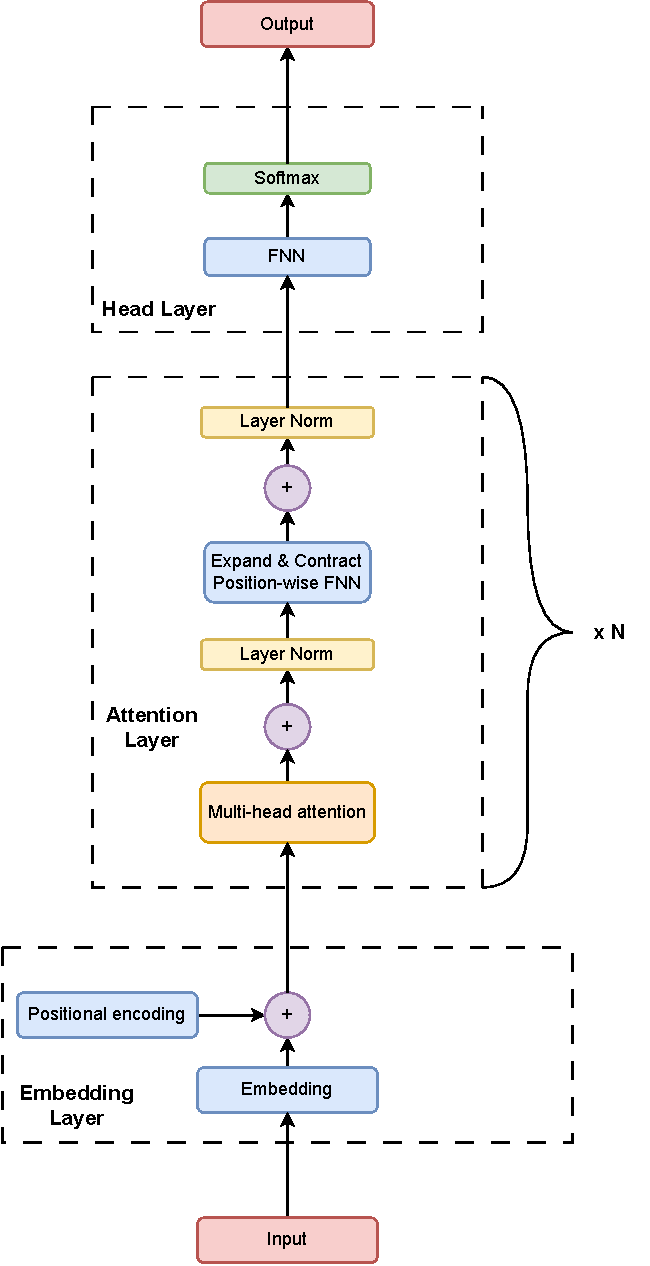
\includegraphics[width=0.7\linewidth]{img/transformer/trans_architecture.pdf}
    \caption{Transformer architecture without Dropout blocks for clarity.}
    \label{fig:transformer}
\end{figure}

The architecture of the transformer can be seen at \autoref{fig:transformer}.
The key components are
\begin{itemize}
    \item Embedding layer
    \item Multi-Head Attention Block
    \item Head layer
\end{itemize}
We will now describe each of them in detail.
\subsubsection{Embedding Layer}
The first layer of the transformer is an embedding layer, it takes the input text encoded as a vector $\mathbf{x} \in R^{n}$, with values in the range $[0, V)$, where $V$ is the vocabulary size.
The embedding layer embeds each vector element into vector space by employing a learnable matrix $\mathbf{E} \in R^{V, d}$, where $d$ is the arbitrary embedding dimension.
To encode the word's position in the sentence, we add a learnable positional embedding $\mathbf{P} \in R^{n, d}$.
Thus, the output of the embedding layer is given by
\begin{equation*}
    \mathbf{O} = \operatorname{OneHot}(\mathbf{x}) \cdot \mathbf{E} + \mathbf{P}
\end{equation*}
where $\operatorname{OneHot}(\mathbf{x})$ is a matrix of one-hot vectors, where each row corresponds to the one-hot vector of the corresponding element in $\mathbf{x}$.
This makes the model only accept fixed-length inputs.~\footnote{The original paper allowed for variable length inputs by employing a different strategy for positional encoding.}

\subsubsection{Self-attention}
Self-attention is a key mechanism of transformer architecture.
The Queries ($\mathbf{Q}$), Keys ($\mathbf{K}$), and Values ($\mathbf{V}$) matrices are computed from inputs as follows
\begin{align*}
    \mathbf{Q}                                             & = \mathbf{X} \mathbf{W_q}                  \\
    \mathbf{K}                                             & = \mathbf{X} \mathbf{W_k}                  \\
    \mathbf{V}                                             & = \mathbf{X} \mathbf{W_v}                  \\
    \text{where } \mathbf{W_q}, \mathbf{W_k}, \mathbf{W_v} & \in R^{d, d} \text{are trainable matrices}
\end{align*}
The output of the self-attention layer is then computed as follows~\footnote{The dimension hidden state of self-attention can be different from the embedding dimension. We use the same for simplicity.}
\begin{align*}
    \mathbf{O} & = \operatorname{softmax}\left(\frac{\mathbf{Q} \mathbf{K}^T}{\sqrt{d}}\right) \mathbf{V} \\
    \label{eq:attention}
\end{align*}
The intuition behind the self-attention is that by doing a scalar product between query and key vectors,
the model learns to focus on the most relevant parts of the input.
Such parts will then have the highest weight in the output in values multiplication.

\subsubsection{Multihead attention}
The multi-head attention is an extension of self-attention.
Instead of doing just one attention, we do multiple attentions in parallel, every attention with different Query, Key and Value matrices.
The outputs are then concatenated and passed through a linear layer.

\subsubsection{Head Layer}
Head Layer is task-dependent, as its task is to convert the transformer's output to the desired output.

\subsubsection{Benefits and Drawbacks}
\label{sec:benefits-and-drawbacks}
What transformers mostly improved were two things:
\begin{itemize}
    \item Capturing of long-range dependencies.
    \item Parallelization of the model. Unlike \acp{rnn}, we don't process a single input at a time,
          but all of them in parallel. This allows for much faster training.
\end{itemize}
However, advantages haven't come without a cost. One of the biggest problems with transformers
is their memory complexity. The self-attention layer requires $O(n^2)$ memory and $O(d \cdot n^2)$ time complexity.
This limits the use of transformers to lower-length inputs. However, much work has been done in recent years to mitigate this issue~\parencite{zhuangSurveyEfficientTraining2023}.

\subsection{Transfer Learning}
\label{sec:transfer-learning}
Transfer learning is a technique that allows using knowledge gained from one task to solve another.
The popular method of transfer learning is fine-tuning. To fine-tune a model, we take a pre-trained model (\textbf{backbone})
and train it on a new task with a new task-specific head.

\subsection{\acl{lm}}
The popular backbone models are \acfp{lm}. The goal of the \ac{lm} is to predict the next token in a sentence.
Due to the simplicity of the task, it can be trained in an unsupervised manner allowing for large-scale training.
The approach is relatively old and was used even before the transformers with \acp{rnn}~\parencites{daiSemisupervisedSequenceLearning2015}{petersSemisupervisedSequenceTagging2017}.
The transformers allowed this method to scale to much larger datasets and models.

\subsection{BERT}
\textbf{Bert}~\parencite{devlinBERTPretrainingDeep2019a} is a successor to the previous attempts of training transformer \acp{lm}, namely ELMo~\parencite{petersDeepContextualizedWord2018} and GPT~\parencite{Radford2018ImprovingLU}.
The main difference between BERT and previous methods is that it uses a bi-directional encoder.
Previous work used a single-direction encoder; \ac{lm} model only attending to the left or right context.
The bi-directional encoder allows the model to attend to the context in both directions.
That's achieved by the \acf{mlm} optimization objective.

\subsubsection{\acl{mlm}}
\label{sec:masked-lm}
The goal of the \ac{mlm} is to predict the masked tokens in the text.
The model is trained to predict the masked words by taking input tokens and replacing some of them with a special token \verb|[MASK]|.
As the model won't see the mask tokens during inference, some tokens in the input are replaced with random tokens from the vocabulary instead of the mask token.

\subsubsection{\acl{nsp}}
To improve the model's ability to capture relationships between two sentences,
the BERT further uses the \acf{nsp} objective.
Given two sentences, the model is trained to predict if the second sentence follows the first in the original text.

\subsubsection{Input Representation}
The BERT uses a WordPiece tokenization~(\autoref{sec:wordpiece}) to convert the input text to tokens.
Apart from learned tokens, BERT introduces three special tokens:
\begin{enumerate}
    \item \verb|[CLS]| - Token appended to start of token sequence. The predicted output is based on the hidden state of this token.
    \item \verb|[SEP]| - The token appended to the end of the token sequence.
    \item \verb|[MASK]| - The token that is used for masking in \autoref{sec:masked-lm}.
\end{enumerate}


\subsubsection{Bert-base and Bert-large}
\begin{table}[h]
    \centering\footnotesize\sf
    \begin{tabular}{lrr}
        \toprule
        {}                        & BERT-base & BERT-large \\
        \midrule
        Hidden size               & 768       & 1024       \\
        Number of layers          & 12        & 24         \\
        Number of attention heads & 12        & 16         \\
        \bottomrule
    \end{tabular}
    \caption{Comparison of BERT-base and BERT-large.}
    \label{tab:bert-base-large}
\end{table}

Bert model exists in two versions: BERT-base and BERT-large;
they differ by the number of layers and hidden layer size as seen in~\autoref{tab:bert-base-large}.


\subsection{RoBERTa}

\begin{table}[h]
\centering\footnotesize\sf
    \begin{tabular}{lrr}
        \toprule
        {}              & BERT                                    & RoBERTa            \\
        \midrule
        Batch size      & 256                                     & 512                \\
        Sequence length & 128 tokens (90\%) and 512 tokens (10\%) & 512 tokens (100\%) \\
        Tokenization    & WordPiece                               & \ac{bpe}           \\
        Data            & 16 GB                                   & 160 GB             \\
        Objective       & \ac{mlm} + \ac{nsp}                     & \ac{mlm}           \\
        \bottomrule
    \end{tabular}
    \caption{Comparison of BERT and RoBERTa.}
    \label{tab:bert-roberta}
\end{table}

\textbf{RoBERTa}~\parencite{liuRoBERTaRobustlyOptimized2019} is a further refinement of the BERT model.
It doesn't change the model's architecture, but instead changes how the model is trained.
The key differences are displayed in~\autoref{tab:bert-roberta}.

\subsection{GPT-3}
\textbf{GPT-3} is a family of models introduced by \textcite{brownLanguageModelsAre2020b}.
Due to them being developed by \textbf{OpenAI}~\footnote{\url{https://openai.com/}}, they are not publicly available and not much is known about them.
As per \textcite{brownLanguageModelsAre2020b}, the GPT-3 models are transformer-based \acp{lm} with parameters ranging from 125M to 175B, trained on
a large multi-lingual dataset with more than 570GB of text. The tokenizer is based on the \ac{bbpe}~(\autoref{sec:bbpe}) algorithm.
To solve efficiency issues~(\autoref{sec:benefits-and-drawbacks}), the model also employs sparse attention modification~\parencite{childGeneratingLongSequences2019}.
The OpenAI offers paid fine-tuning and inference of the derivatives of GPT-3 models, but no information about the models themselves.

\subsection{Multi-linguality of \aclp{lm}}
\label{sec:multilinguality}
Both BERT and RoBERTa are trained exclusively on English data. To allow extension to other languages,
multi-lingual models were introduced. Namely, XLM~\parencite{lampleCrosslingualLanguageModel2019a}, XML-R~\parencite{conneauUnsupervisedCrosslingualRepresentation2020}
and m-BERT~\parencite{piresHowMultilingualMultilingual2019}. GPT-3 models could also be considered a multi-lingual model as 7\% of the training data is in non-English languages
and show great results on translation tasks to English.

While the models have shown multi-lingual capabilities,
they possess two major drawbacks:
\begin{itemize}
    \item The embedding layer must be substantial to accompany many languages.
    \item Length of tokenized sequences tends to be very long due to multi-lingual tokenization training.
\end{itemize}
It has been also shown by \cite{strakaRobeCzechCzechRoBERTa2021} and \cite{scheibleGottBERTPureGerman2020} that the
mono-lingual models can still outperform the multi-lingual models on certain target language tasks, while being significantly smaller.

\subsection{Czech Mono-lingual \aclp{lm}}
\begin{table}[h]
    \resizebox{\linewidth}{!}{%
        \centering\footnotesize\sf
        \begin{tabular}{lrrrrr}
            \toprule
            Model                                                                            & Base Model    & Tokenizer & Vocab & Training Data           & \# Params \\
            \midrule
            M-BERT~\parencite*{devlinBERTPretrainingDeep2019a}                               & BERT-base     & WordPiece & 120k  & Wiki, 104 langs         & 179M      \\
            XLM-RoBERTa-base~\parencite*{conneauUnsupervisedCrosslingualRepresentation2020}  & RoBERTa-base  & \ac{spm}  & 250k  & CC, 100 langs (2TB)     & 278M      \\
            XLM-RoBERTa-large~\parencite*{conneauUnsupervisedCrosslingualRepresentation2020} & RoBERTa-large & \ac{spm}  & 250k  & CC, 100 langs (2TB)     & 560M      \\
            \midrule
            Czert~\parencite*{sidoCzertCzechBERTlike2021}                                    & BERT-base     & WordPiece & 40k   & Syn+Wiki+News (37GB)    & 110M      \\
            RobeCzech~\parencite*{strakaRobeCzechCzechRoBERTa2021}                           & RoBERTa-base  & \ac{bbpe} & 52k   & Syn+Wiki+Czes+W2C       & 126M      \\
            FERNET-C5~\parencite*{leheckaComparisonCzechTransformers2021}                    & BERT-base     & \ac{spm}  & 100k  & C5 (93GB)               & 164M      \\
            FERNET-News~\parencite*{leheckaComparisonCzechTransformers2021}                  & RoBERTa-base  & \ac{bbpe} & 50k   & News Corpus (21GB)      & 124M      \\
            Small-E-Czech~\parencite*{kocianSiameseBERTbasedModel2021}                       & Electra-base  & WordPiece & 30k   & Internal corpus (253GB) & 13 M      \\
            \bottomrule
        \end{tabular}
        \caption{Table comparing multi-lingual and Czech mono-lingual models.
            Electra-base~\parencite*{clarkELECTRAPretrainingText2020} is a transformer architecture trained
            with discriminative pre-training rather than generative. \textit{CC} stands for Common Crawl.
            The table is a slightly modified version of \textcite[Table 2]{leheckaComparisonCzechTransformers2021}.}
        \label{tab:czech-monolingual}
    }
\end{table}
Czech pre-trained \acp{lm} are depicted in \autoref{tab:czech-monolingual}. We will now briefly
describe Fernet-News and RobeCzech models, as we will use them in our experiments.

\subsubsection{Fernet-News}
\label{sec:fernet}
Developed at the \textit{University of West Bohemia in Pilsen}, Fernet-News is a Czech RoBERTa model trained on
over 3.3B words of Czech text. The training data mainly consists of Czech news articles and transcripts of TV and radio shows.
The tokenizer is \ac{bbpe} based, containing 50k tokens.
The model was trained for 700k steps with a batch size of 2048 and a learning rate of 1e-4.
Unlike the original RoBERTa model, the model was first pre-trained on 128-long inputs for 600k steps, followed by 100k steps
of 512-long inputs.

\subsubsection{RobeCzech}
\label{sec:robe-czech}
Developed at the \textit{Charles University in Prague}, RobeCzech is a Czech RoBERTa model trained on over
4.1B tokens of Czech text. The training data are gathered from 4 different sources:
\begin{itemize}
    \item \textbf{SYN v4}~\parencite*{11234/1-1846} - a corpus of contemporary (written) Czech texts. It contains a large proportion
          of journalistic texts from the Czech presses.
    \item \textbf{W2C}~\parencite*{11858/00-097C-0000-0022-6133-9} - corpora containing texts from Wikipedia and web. As it contains 120 languages, only the Czech part was selected.
    \item \textbf{Czes}~\parencite*{11858/00-097C-0000-0001-CCCF-C} - a corpus of Czech magazine and newspaper articles.
    \item \textbf{Wiki}~\parencite*{strakaRobeCzechCzechRoBERTa2021} - Wikipedia extracted texts.
\end{itemize}
The vocabulary was created with \ac{bbpe} and contains 51960 tokens.
The model was trained for 91k steps with a batch size of 8192 and a learning rate of 7e-4.



\chapter{Dataset}
\label{chap:math}

We first had to find a suitable dataset to evaluate the scientific question.
Thus we consulted literature and the internet to find a dataset that would suit our needs.
 We needed a News dataset that would suffice these requirements:

\begin{itemize}
    \item Contains content of the article for each sample
    \item Partially contains category, authors, publication date, publication server
    \item Size of at least 200k samples
    \item Language: Czech
\end{itemize}


The closes to our requirements we found were:
\begin{itemize}
    \item \cite{strakaSumeCzechLargeCzech2018a} - 1M czech news articles.

        While sufficiently large and in the correct language, 
        it doesn't contain either category, not author metadata. 
        However, the paper provides valuable information about dataset extraction
        and cleaning of the dataset.
    \item \cite{misraNewsCategoryDataset2022} - 210k english news articles.

        While it contains both category and author metadata,
        the language is English, and the dataset doesn't have the content of the articles.
end{itemize}

As neither dataset suited our needs, we created our dataset.


\section{Dataset creation}
\label{sec:dataset-creation}

\subsection{Data source}
We initially decided to collect the data from these news servers:
\begin{itemize}
    \item Seznamzpravy.cz
    \item Irozhlas.cz
    \item Novinky.cz
    \item Aktuálně.cz
    \item Idnes.cz
    \item Ihned.cz
    \item Deník.cz
\end{itemize}

These sources were chosen due to their popularity and high amount of articles.
To get articles, we had two options:
\begin{enumerate}
    \item Use a web spider to crawl the live website.
    \item Use a web archive that would contain crawled articles.
\end{enumerate}
We chose the second option because crawling live websites is tricky,
as the servers would be too fast to block the crawler due to too many requests.
The second problem is that we would probably not be able to get as many articles as
if we used the second option since there might be no links to old articles anymore.

\subsection{Webarchive}
As a web archive, we chose a CommonCrawl~\cite{CommonCrawl}. 
CommonCrawl is an open-source project crawling the web and storing the data. 
The data are stored as a WARC\todo{Should I somehow cite this ?} files in Amazon's S3 storage.
 The data can then be queried using Amazon's big data tools or CommonsCrawl's API.
The data stored in the archive have been collected since 2008 with various frequencies,
but since 2014 they have been collected monthly.

\subsection{Data extraction}
\subsubsection{CC Extractor}
To extract the data, we built a program that can extract the data from a CommonCrawl
 based on the URL, data, etc\dots. The program was 
created strongly emphasizing scalability and realability\todo{I Guess I should explain these terms?}.
It's separated into two parts:
\begin{enumerate}
    \item Aggregator - 
    Extracts links from CommonCrawl API for specified URLs and sends them to a Processor.
    \item Processor - 
    Loads the WARC data from S3 and extracts the requested metadata.
    For extraction, we used python's beautifulsoup library.
\end{enumerate}
Both of them can be scaled based on the needs.
The connection between the Aggregator and processor can be made using various middlewares.
As of now, the used middleware is ActiveMQ Aremis~\cite{ActiveMQ}.
When the Aggregators send links to Processors,
they are filtered based on the normalized version(URL without query, duplicated '/' etc\dots).
\todo{Should I go more in-depth with the description ?}
\subsubsection{Extraction}
We have done extraction on 12.12.2022.
We set the extractors to only output articles in which the processor successfully
extracted the content and headline.
We set the aggregators to process crawls from 1.1.2008 to 31.8.2022.
We used the~\cite{UFALAIC} for the deployment of the extractor. 
We run one aggregator and four processors for each server,
totaling seven extractors and 28 processors.
As for orchestration, while the program has working docker support,
the cluster doesn't support it, and thus we used shell scripts for deployment.
The 49M URLs were processed, of which the processor received 82M
and successfully processed 31M articles.

Once we extracted the data, we started with filtering and postprocessing.
\subsection{Filtering}

Filtering was done in following steps:
Precise amounts of articles filtered can be seen in



\subsection{Ihned.cz articles}
Similar to~\cite{strakaSumeCzechLargeCzech2018a}, we found that the Ihned.cz articles contained
a high number of paywalled articles and overall didn't contain many samples.
We thus decided to drop it.

We proceeded with filtering, which we did in these three steps:
\subsection{CZ filtering}
Since we were interested in Czech articles, we decided to filter out articles
not in the Czech language. For this purpose,
we used FastText Language detection model~\cite{joulinFastTextZipCompressing2016,joulinBagTricksEfficient2016}. The model was run on each line article of content which. This allowed us to interpret fraction of lines that were predicted as czech as confidence of article being czech.
We inspected the articles with lower confidence, and the most occurring problems were:
\begin{enumerate}
    \item Articles in Ukraine language on Seznamzpravy.cz, due to the recent war in Ukraine
    \item Articles with a list of sports results where most texts were
    the result, team, and match highlights.
    \item Articles with comparison tables, e.g., mobile comparison
    \item Galeries, there were few articles with galleries of pictures or videos with little text.
    \item English articles on Idnes.cz and Irozhlas.cz
\end{enumerate}
We then empirically chose 0.75 as a threshold for confidence.

\subsubsection{Filtering by Article Statistics}
The main goal of this step was to filter out either wrongly parsed
or non-news articles(plain sports results, weather, tables, videos/photos\dots).
We thus inspected article content based on several properties
and set the following thresholds to remove unwanted characters:
\begin{enumerate}
    \item General:
    \begin{enumerate}
        \item Content length - $(400, \inf)$
        \item Headline length - $(20, \inf)$
        \item Brief length - $(40, \inf)$
        \item Date - $(1.1.2000, 31.8.2022)$
    \end{enumerate}
    \item Content:
    \begin{enumerate}
        \item Average word length - $(4.0, \inf)$
        \item Num of words / Lenght - $(0.11, 0.22)$
        \item Non-alphanumeric characters / Length - $(0, 0.045)$
    \end{enumerate}
\end{enumerate}

During the inspection, we further found the following problems:
\begin{enumerate}
    \item Headline cuts

        When observing articles with short headlines, we found that the headlines 
        were cut in the middle of words.
        It was because the extractor had a function that would remove anything after `-'. 
        In headlines, it was supposed to prevent the bloat like `- Aktuálně.cz'. However,
        we didn't anticipate this would also remove words like start-up, etc\dots.
        We removed this rule and reran the whole extraction.
    \item Article character length

        When observing article length at Novinky.cz and Seznamzpravy.cz,
        we found many articles with sizes of less than 100 characters.
        We found that this was due to an extraction error. 
        For these two sites, we were extracting content by CSS classes.
        However, we didn't include all possible classes;
        thus, sometimes extractor extracted only headers. 
        We tried to fix the problems by adding more classes and generalizing the CSS selectors,
        reducing the issue but not eradicating it. We thus decided to resolve this problem
        by the content length rule.

    \item Brief/Headline length drops

        When inspecting Aktualne.cz we found that headlines
        had steep drops in several samples at specific headline lengths (55, 60, 85).
        However, we haven't found any problems with such headlines.
        We assume these inconveniences result from internal rules for writers at Aktualne.cz.
\end{enumerate}

\subsubsection{Filtering by headline content}
As in \cite{strakaSumeCzechLargeCzech2018a}, many articles
contained prefixes at headlines like 'VIDEO: ', 'FOTO: ', 'GALERIE: ' etc\dots.
Since we were interested in the articles and not galleries,
we dropped the articles with prefixes that indicate not a non-article.
However, unlike \cite{strakaSumeCzechLargeCzech2018a}, we haven't removed these prefixes
in non-filtered headlines/briefs.




\subsubsection{Headline/Brief/Content dedupliation}
The last filtering round removed articles with identical briefs, headlines, or content.

We were afraid that this would also affect the article across different serves.
It turned out that the deduplication only deleted around 3K articles
because of cross-server duplicates.

When choosing which duplicate to use, we took the one with the most metadata filled
or the longer article length.

Therefore, every Brief/Content/Headline is unique in the dataset.

\subsection{Data Augmentation and Postprocessing}

\subsubsection{Category}
\label{sec:category}
Due to the wide variety of collected data, we had to normalize categories.
After extraction, we got a total of 3383 categories.
Since there was considerable overlap between each category,
we selected 25 categories among the most popular ones.
We focused on choosing the classes with the most samples
while ensuring a small overlap between selected categories.
That's why we dropped categories like Zprávy, Tipy, Vaše zprávy, Ostatní, etc\dots,
even though they had a high amount of samples.


We then mapped from the remaining categories to these 25 categories if such a mapping was possible.
Examples of such mappings are:
\begin{enumerate}
    \item Football, Tennis, Biatholon\dots $\rightarrow$ Sport
    \item Praha, Domažlicko, Ústecko\dots $\rightarrow$ Domácí
    \item Ona, Ženy, Móda\dots $\rightarrow$ Životní styl
\end{enumerate}


\subsubsection{Authors}
\label{sec:authors}
After extraction, there were 27K unique authors.
The obvious problem was that not all authors were people.
Surprisingly, the most prevalent were the news institutions: ČTK, IDnes, MF DNES, etc\dots.
There were also many nicknames we couldn't decode, companies,
and common names like Redakce, externí, etc\dots.

We thus employed heuristics and manual filtering 
to mitigate these problems and ended up with 11K authors.
As for postprocessing, we removed occupation, academic titles, and mysterious form names.

\subsubsection{Gender and cumulative gender}
\label{sec:gender}
As gender was not provided in articles, we had to guess it for names.
As \cite{seboPerformanceGenderDetection} suggests,
we used \cite{NamsorNameChecker} as per \cite{seboPerformanceGenderDetection}
it is one of the most accurate. 

For cumulative gender, we used the following rules:
\begin{enumerate}
    \item If all authors of the article are MAN $\rightarrow$ MAN
    \item If all authors of the article are WOMAN $\rightarrow$ WOMAN
    \item MIXED otherwise
\end{enumerate}

\subsubsection{Content, Brief, Headline Postprocessing}
We used the following postprocessing steps for content, brief, and headline:
\begin{enumerate}
    \item Replace '\\n','\\r','\\t' with spaces
    \ Truncate item spaces
    \item Convert named and numeric character references to Unicode,
    e.g., '\&\#x2013'; to \textendash.
    \item Normalize Unicode characters to their base combined form.
\end{enumereate}
As for Brief and Headline, we capitalized the first letter
and added a dot at the end if there wasn't one.

\subsection{Splits}
Since we were interested in predicting the future,
we decided to split the data into train, validation, and test set based on the published date.

The sets are, therefore, not random but ordered by published date. Train set having the earliest, while test the latest.
If the sample didn't have a published date, we randomly assigned it to one of the sets.
The ratio between the sets is $85:7.5:7.5$.
\section{Dataset summary} 
\label{sec:dataset_summary} 
\begin{table}
% uncomment the following line if you use the fitted top captions for tables
% (see the \floatsetup[table] comments in `macros.tex`.
%\floatbox{table}[\FBwidth]{
\centering\footnotesize\sf
\begin{tabular}{llrl}
\toprule
Server & Size & Unique Authors & Categories & Date Range & Article words \\
Seznamzpravy.cz & 65472 & 382 & 11 & 14.9.2016 - 6.8.2022 & 443
Denik.cz & 664133 & 2497 & 18 & 27.3.2007 - 6.8.2022  & 332 
Idnes.cz & 295840 & 4385 & 21 & 3.1.2000 - 9.8.2022 & 423
Irozhlas.cz & 167588 & 1900 & 8 & 8.7.2000 - 25.6.2022 & 287
Aktualne.cz & 112960 & 633 & 19 & 26.10.2005 - 6.8.2022 & 468
Novinky.cz & 321417 & 2518 & 17 & 20.12.2002 - 6.8.2022 & 274
\midrule
Cumulative & 1627410 & 10930 & 25 & 3.1.2000 - 9.8.2022 & 362 \\
\bottomrule
\end{tabular}
\end{table}



% \begin{table}
% % uncomment the following line if you use the fitted top captions for tables
% % (see the \floatsetup[table] comments in `macros.tex`.
% %\floatbox{table}[\FBwidth]{
% \centering\footnotesize\sf
% \begin{tabular}{llrl}
% \toprule
% Phase & Seznamzpravy.cz & Denik.cz & Idnes.cz & Irozhlas.cz & Aktualne.cz & Novinky.cz
% Found CC Articles & 280015 & 13520220 & 26692819 & 1015624 & 1790014 & 3808423
% Extracted & 664133 & 2497 & 18 & 27.3.2007 - 6.8.2022  & 332 
% CZ + Stats + Brief Filter & 295840 & 4385 & 21 & 3.1.2000 - 9.8.2022 & 423
% Brief/Content/Headline Filter & 167588 & 1900 & 8 & 8.7.2000 - 25.6.2022 & 287
%  & 112960 & 633 & 19 & 26.10.2005 - 6.8.2022 & 468
% Novinky.cz & 321417 & 2518 & 17 & 20.12.2002 - 6.8.2022 & 274
% \midrule
% Cumulative & 1627410 & 10930 & 25 & 3.1.2000 - 9.8.2022 & 362 \\
% \bottomrule
% \end{tabular}
% \end{table}

\section{Task description}
Overall we are interested in 4 tasks with this dataset:

\subsection{Article category prediction}

\subsection{Article server prediction}

\subsection{Article day prediction}

\subsection{Aritcle gender prediction}


\chapter{Experiments}
\label{chap:experiments}
To evaluate the research question we have conducted in total 9 experiments for every task.
We categorize experiments into 4 groups: Human performance, Baseline, Backbone models and Fine-tuning methods.

\section{Human performance}
\label{sec:human}
To evaluate human performance, we let 5 evaluators classify the articles on Test-human set (see \autoref{enum:test-human}).

\section{Baseline}
For a baseline, we have used Multi-class Logistic Regression with TF-IDF features.
TF-IDF features setting was:
\begin{enumerate}
    \item Tokenization method: lowercased text with MosesTokenizer\footnote{https://pypi.org/project/mosestokenizer/}
    \item Maximum document frequency: 1\%
    \item Ngrams: 1-2
    \item Minimum document frequency: 90 documents
\end{enumerate}
Similar to \cite{strakaSumeCzechLargeCzech2018a} we have added following additional features:
\begin{enumerate}
    \item Number of words
    \item Number of words with only non-alphabetic characters
    \item Number of uppercase words
    \item Number of digits words
    \item Number of capitalized words
\end{enumerate}


We run a grid search over the following hyperparameters:
\begin{enumerate}
    \item Inverse Regularization term: $1, 10, 100, 1000$
\end{enumerate}
We selected the best model based on the f1-macro score on the validation set.
As for the solver, we have used SAGA (\cite{defazioSAGAFastIncremental2014})
 implementation from Scikit-learn library\footnote{https://scikit-learn.org}.
with max iterations set to 800 and early stopping tolerance set to 0.001.
With this setting, we created 2 models; \textbf{LR-BASE-40} with 40k features
 and \textbf{LR-BASE-200} with 200k features.

\section{Backbone models}
\label{sec:backbone}
For backbone models, we have used \textbf{RobeCzech}, \textbf{Fernet-News}, and \textbf{GPT-3}.
We chose RobeCzech and Fernet-News as performed well in classification tasks while being reasonably big.
The GPT-3 was chosen as we were interested in its capabilities due to its size.

\subsection{RobeCzech and Fernet-News}
\label{sec:robe-czech}
For finetuning we mostly followed the hyperparameters
recommend at \cite{sunHowFineTuneBERT2020}.
As for architecture, we took the backbone model and replaced the head as shown in: \autoref{fig:class-tune}.

\begin{figure}[h]
    \centering
    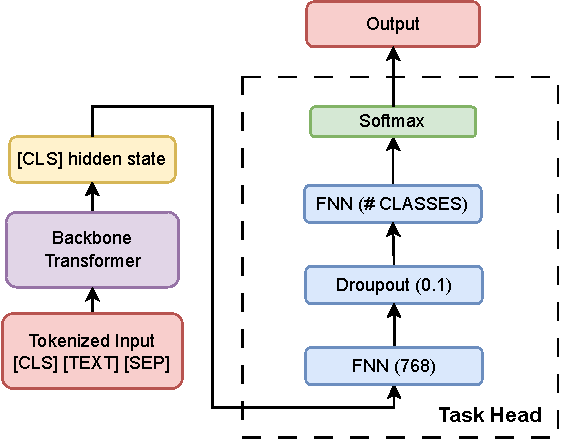
\includegraphics[width=0.7\linewidth]{img/transformer/fine_tune.pdf}
    \caption{Fine-tuning architecture for the classification task.}
    \label{fig:class-tune}
\end{figure}

We have used the following hyperparameters:
\begin{enumerate}
    \item Effective Batch size
    \footnote{By effective batch size we mean 
    $\text{gradient accumulation steps} \times \text{number of devices}
    \times \text{batch size}$
    }: 48
    \item Number of epochs: 2
    \item Sequence length: maximum 512 tokens with dynamic padding per batch
    \item Weight decay: 0
    \item Optimizer: AdamW with epsilon 1e-8, beta1 0.9, beta2 0.999.
    \item Scheduler: Linear warmup with 0.1 warmup ratio
    \item Unfrozen layers: 12
    \item Truncation: First 512 tokens
    \item Unfrozen Embeddings: False
\end{enumerate}
To find the learning rate (lr), we run a grid search for each model and task with following values: $3e-5, 4.5e-5, 7.5e-5$.
Grid search only run for 0.4 epoch and lr with the best validation f1-macro score was selected.
For implementation, we have used \textit{Pytorch Lightning 2.0}, \textit{Huggingface Transformers 4.24} and \textit{Pytorch 2.0.0}.
The training was done on Ufal AIC cluster\footnote{https://aic.ufal.mff.cuni.cz/} on a single GeForce RTX 2080 Ti.

\subsection{GPT-3}
\label{sec:gpt-3}
We have chosen Ada version of GPT-3 as it is the cheapest.
Ada costs $0.00004\$/1k$ tokens for finetuning and $0.00016\$/1k$ tokens for a generation.
As the model architecture is not modifiable, the finetuning works
as text generation fine-tuning.
Thus we only provide query: Text of article and text completion: Class.
To save the cost we fine-tuned in a multi-task setting.
Thus for every task, we created a label in the format: \textit{Full\ Server Name} \textit{Category} \textit{Gender} \textit{Day of week}.

Example of the label:
\begin{quotation}
    \textit{Idnes.cz Sport Muž Pondělí}
\end{quotation}

The Ada model takes a maximum of 2048 tokens, we thus truncated documents to 1400 characters.
To save the costs we used Train-small (see \autoref{enum:train-small}) for finetuning and
Test-small (see \autoref{enum:test-small}) for inference.
We then finetuned for 2 epochs.
For comparison, we also additionally fine-tuned and evaluated the above models on the same dataset.

\section{Fine-tuning}
\label{sec:finetuning}
We were interested in ways to improve the performance of finetuning without changing the backbone model.
We tried 3 approaches mainly inspired by \cite{howardUniversalLanguageModel2018a} and \cite{sunHowFineTuneBERT2020}.
Note that \textbf{ULMFiT} is RNN architecture and thus its findings might not apply to transformers.
All the experiments were done on \textbf{RobeCzech} model.

\subsection{Truncation}
\label{sec:truncation}
The base models are trained with truncation of the first 512 tokens as it was shown
the most effective by \cite{sunHowFineTuneBERT2020}. Due to the nature of task,
we hypothesized that the last part might contain more relevant information as:
\begin{quotation}
    Pro Idnes.cz Jana Křížová
\end{quotation}
We thus tried to truncate the text by taking the last
512 tokens.

\subsection{Task modeling}
\label{sec:task-modeling}
Both \cite{howardUniversalLanguageModel2018a} and \cite{sunHowFineTuneBERT2020} found that further LM modeling on
task dataset can improve the performance. We thus tried to use the same approach on our dataset.

\subsection{Gradual unfreezing with discriminative learning rates}
\label{sec:gradual-unfreezing}
This idea was inspired by \cite{howardUniversalLanguageModel2018a}.
When doing the gradual unfreezing, we unfreeze the layers in groups until all the layers are unfrozen.
The discriminative learning rate is a technique where the learning rate is different for each layer.
We set the discriminative factor to $0.95$ as in \cite{sunHowFineTuneBERT2020}.
The gradual unfreezing is not well described in ULMFiT, thus we tried two approaches:
\begin{enumerate}
    \item GradDLR-12 Unfreeze 1 layer per epoch, starting from the last layer, and run for 12 epochs.
    \item GradDLR-24 Unfreeze 1 layer per epoch, starting from the last layer, and run for 24 epochs(12 epochs in the full unfrozen state).
\end{enumerate}
The epoch lengths are adjusted, so that the total number of optimizer steps stays the same (full 2 epochs).

For both approaches, we unfreeze the classifier layer at epoch 0 with lr decaying from $1e-3$ to $ 5e-5$.
The first unfrozen layer has lr peak at $3e-5$. The remaining layers are adjusted based on the discriminative learning rate.
Each unfrozen layer has its scheduler with the same setting as base model tuning (\autoref{sec:backbone}). However, it start scheduling when the layer was
unfrozen.
The reaming setting stays the same as in base model tuning (\autoref{sec:backbone}).


\ifEN
\chapwithtoc{Bibliography}
\else
\chapwithtoc{Seznam použité literatury}
\fi

\printbibliography[heading=none]


\appendix

% if your attachments are complicated, describe them in a separate appendix
%\include{attachments}

\openright
\end{document}
